\chapter{Applications and Use Cases}
\label{chapter:applications}
\epiquote{If your only tool is a hammer then every problem looks like a nail.}{Abraham Maslow, 1966}

An aspect that has always fascinated me about computer science and information technology is, that it has applications in every conceivable domain. It is this combination of purely technological aspects -- the computational part -- and the domain knowledge, that make this field challenging as well as interesting. Digital transformation -- the act of improving businesses and processing using digital technology \cite{Vial:2019Understanding} -- has been a driving force behind economic activity over the past decades, and while many non-technological factors define digital transformation, optimisation through the application of dispruptive technologiies remains the main incentive behind it.

It is therefore, that we do not want to detach the work presented in this Thesis from its concrete applications and instead aim to motivate it based on real-world scenarios. We do so, by introducing three use-cases, for which we believe that a multimedia database system could fulfill an important function. From these use-cases, we then go on to derive a series of requirements fur such a general-purpose multimedia database.

\section{Use case 1: Interactive Multimedia Retrieval}
\label{section:application_retrieval}

Multimedia retrieval in a broader sense describes the act of finding items of interest in large multimedia collections, wherein ``multimedia'' can refer to any type of modality, such as text, images, videos or audio and any combination thereof. Consequently, a multimedia retrieval system must be able to have a user express their \emph{information need} as a \emph{query} that the system can then use to (ideally) produce the item(s) of interest as a \emph{result}. The process is visualized in \Cref{figure:mr-ideal} and a formal problem definition will be provided in \Cref{chapter:theory_multimedia_analysis_and_retrieval}.

\begin{figure}[tb]
    \centering
    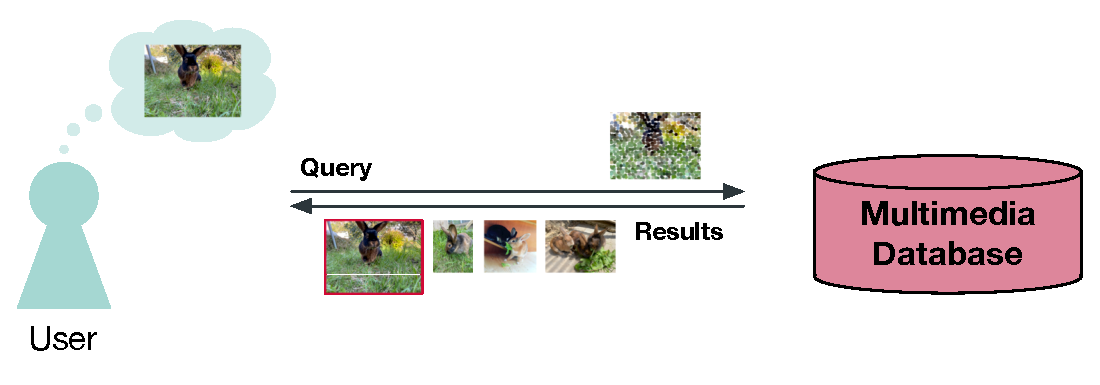
\includegraphics[width=\textwidth]{figures/mr-ideal.eps}
    \caption{The idealised multimedia retrieval problem: A user expresses an information need as a query and the multimedia retrieval system returns matching items from a collection as a resultset, ideally including the desired item.}
    \label{figure:mr-ideal}
\end{figure}

There are many potential applications of the multimedia retrieval problem, but to name a few, one could consider libraries of media items produced by radio or TV stations that must be made searchable \cite{Watanabe:1998Multimedia}, collections of cultural heritage data as maintained by museums, archives and archaeology departments \cite{Tsai:2007Review} or medical image databases containing X-rays or \acrshort{mri} images \cite{Mueller:2004Review}.

What makes multimedia retrieval a challenging problem is the inherently unstructured nature of the data, by which we mean that the raw, (digital) information may not directly reflect the content of the item as a human consumer might perceive or describe it. Let us take, for example, the image of a rabbit the user in \Cref{figure:mr-ideal} is looking for\footnote{On purpose, we do not consider the aspect of reconstructing the image from memory, which makes the problem even more challenging.}. If our task were to describe that image so that we can retrieve it from a large database, we might use terms like ``rabbit'', ``bunny'' or ``grass''. We might assume, judging from the image, that the scene is taking place in a ``garden'' and maybe we notice that the rabbit is currently ``munching'' on a ``leaf'' or ``strain of grass''. We might even know the rabbit's breed or name, if we happened to be its owner.

All of this information is formed based on a series of steps ranging from perception, over interpretation to cognition as illustrated in \Cref{figure:knowledge_formation} and each of these steps is accompanied by a loss or distortion of information \cite{Javanmardi:2021Exploring,Rossetto:2018thesis}, which makes this process highly subjective, giving rise to a series of ``gaps'' that influence the outcome. Most importantly, however, all of the aforementioned descriptions are not explicitly contained in the raw image data, which is merely an array of colour values that constitutes the image and does neither come pre-labeled nor pre-described.

\begin{figure}[tb]
    \centering
    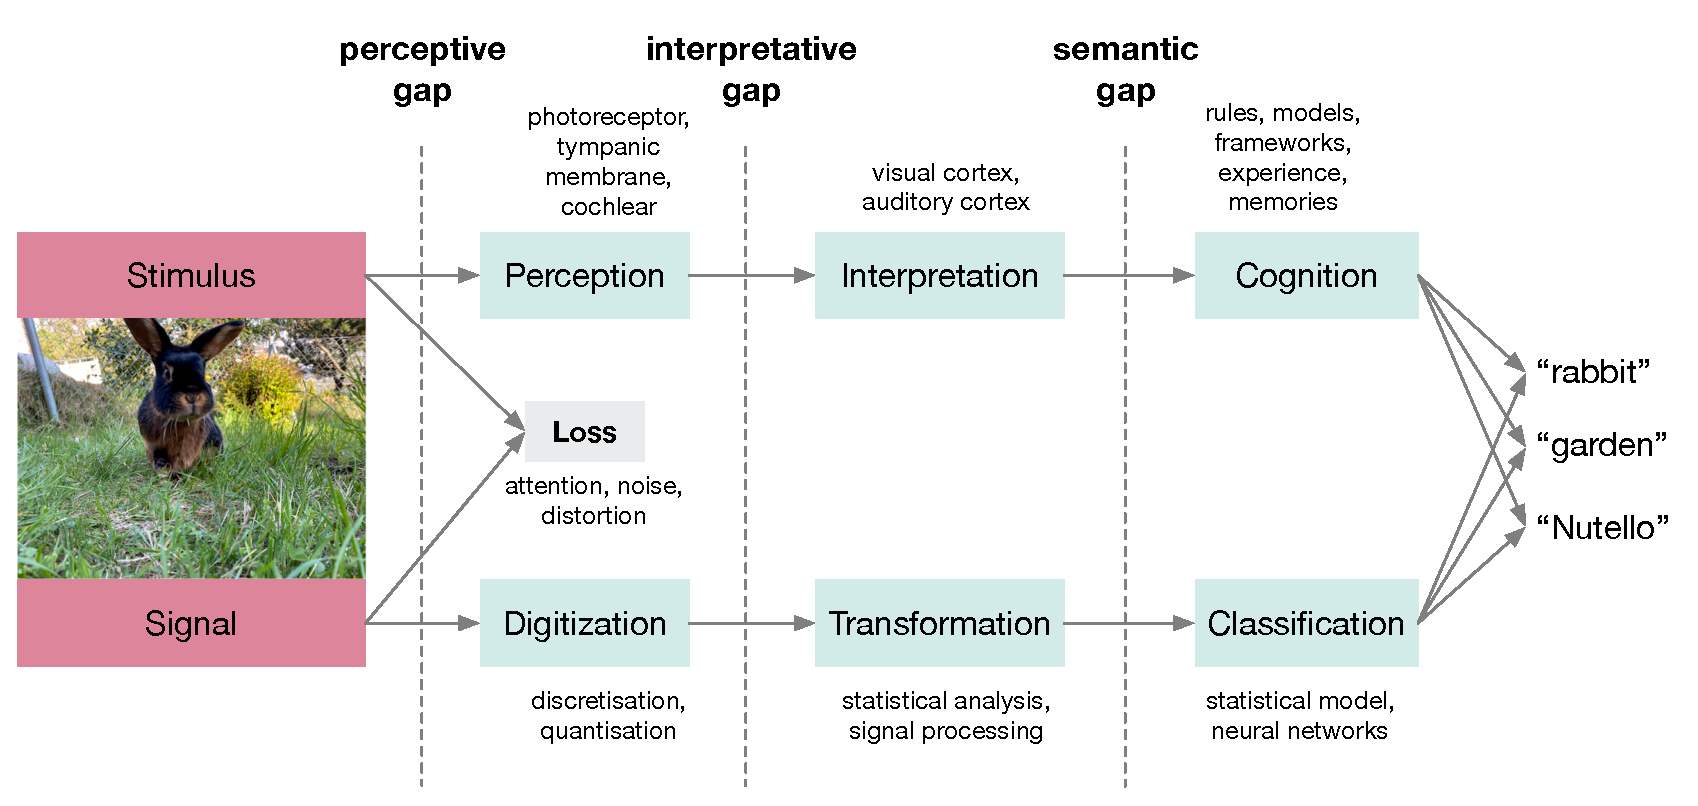
\includegraphics[width=\textwidth]{figures/gaps.eps}
    \caption{A simplified model of knowledge formation in humans (adapted from \cite{Javanmardi:2021Exploring}) and machines.}
    \label{figure:knowledge_formation}
\end{figure}

This impedance mismatch between the content being stored and the information required to find it, is the main challenge that unstructured data brings with it, as opposed to structured data, which consists of retrievable units of information by its nature. Bridging the gaps between the information available and the information we might use to actually search for an item of interest is therefore one of the obstacles to overcome in multimedia retrieval. Over the years, different solutions have emerged:

\begin{description}
    \item[Manual Labeling] The obvious solution is to manually embed the aforementioned labels and descriptions into the multimedia item so that we can use this information to find it at a later point in time. While as of today, this approach is still widely used, it comes with two important disadvantages. Obviously, it remains a subjective task, because as we have argued, the process of forming these labels may yield different results depending on who is assigning them (due to the perceptive, interpretative and semantic gap). Most importantly, though, the task of manual label assignment is laborious and unable to scale with the ever increasing velocity at which multimedia data is produced.
    \item[Automatic Labeling] Recent advances in machine learning have provided us with the ability to automatically label \cite{Redmon:2016You} and even describe \cite{Radford:2021Learning} different types of multimedia through classification. So instead of annotating the content ourselves, we can leave this to pre-trained models that have (at a very high level) a similar mode of operation as a human operator would have, as is illustrated in \Cref{figure:knowledge_formation}. While this solves the problem of scalability, it also remains a subjective task since the process of model training is also prone to the aforementioned gaps found in the data being trained, which can lead to biases \cite{Baer2017:Controlling}. Furthermore, there may be discrepancies between the (mental) model used for classification and the one employed during query formulation, which are typically caried out at different points in time by different people.
    \item[Content-Based Search] The last approach and the one that ``classical'' multimedia retrieval has concerned itself with for decades is that of \emph{content-based search}. Instead of using the higher-level concepts in the form of textual labels, content-based search works with intermediate representations called \emph{descriptors} that are derived from the data directly using signal processing or statistical analysis. These descriptors -- which are often real-valued vectors \cite{Zezula:2006Similarity} -- can then be used to establish a notion of \emph{similarity} between items in a collection and a query. Instead of a list of exact matches, this type of query returns a ranked list of items that match the query well enough. This is called similarity search \cite{Blanken:2007multimedia} and in this context, the query may refer to more than simply textual input. Given the example in \Cref{figure:mr-ideal}, one could use another image of a rabbit as a query (Query-by-Example, \cite{Kelly:1995Query}) or try to create a sketch to find the item of interest (Query-by-Sketch, \cite{Sciascio:1999Content}). One could even come-up with more sophisticated types of queries, such as, querying for poses held by people in an image or video \cite{Heller:2022Multi} or using visual-text co-embeddings \cite{Radford:2021Learning,Spiess:2022Multi} to map textual descriptions to images and vice-versa on the fly.
\end{description}

Decades of research have shown that while individual methods falling into any of the three categories may yield acceptable or even exceptional results, there is clear indication that ultimately, a combination of the three is the most powerful solution, especially, since the exact type of information need is often not known in advance \cite{Rossetto:2020Interactive} \todo{Find source}. Furthermore, because different techniques may perform better or worse depending on the query, we often find that instead of the simple ``issue a query, get a result'' scheme illustrated in \Cref{figure:mr-ideal}, actual multimedia retrieval applications -- which we will henceforth refer to as \emph{interactive multimedia retrieval} -- often involve a back and forth between system and user that involves querying, exploration, browsing, examination of items and query refinement \cite{Lokovc:2019Interactive,Gurrin:2019Invited} as illustrated in \Cref{figure:mr-actual}. This is even explicitly tested at interactive retrieval competitions such as the \acrfull{vbs} \cite{Schoeffmann:2019Video} or the \acrfull{lsc} \cite{Gurrin:2021Introduction}.

\begin{figure}[tb]
    \centering
    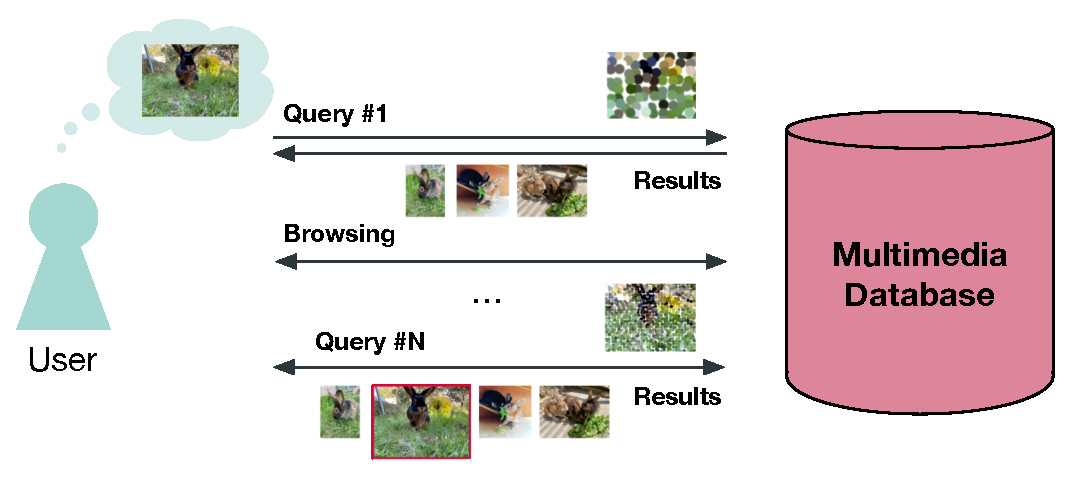
\includegraphics[width=\textwidth]{figures/mr-actual.eps}
    \caption{The interactive multimedia retrieval problem: A continuous back and forth between system and user involving different types of workload as the user tries to find the item of interest through query (re-)formulation, browsing and examination.}
    \label{figure:mr-actual}
\end{figure}
 
These two aspects have important implications for data management systems that support (interactive) multimedia retrieval: Firstly, we have to consider different data- and query models when dealing with information from the aforementioned categories. While searching for labels and textual descriptions at scale can be achieved by the well-established \emph{Boolean retrieval} model, we require the completely different \emph{vector space retrieval} model when dealing with descriptors derived from multimedia data and, ideally, we should have the ability to combine the two in unified queries, as e.g., proposed in the ``multi-stage queries'' presented in \cite{Heller:2020Multi}. This is a problem that has been acknowledged by other authors before \cite{Jonson:2016} and that has been partially addressed, for example, by \cite{Giangreco:2018Database,Giangreco:2016adam,Wang:2021Milvus}. However, all these approaches are limited in how such a combination is possible.

Secondly, any database management system supporting interactive multimedia retrieval workloads must be able to satisfy the different query workloads in a reasonable amount of time, so that the user in the loop must not wait for results too long. This is especially important in timeboxed settings, as for example, evaluation campaigns such as \acrshort{vbs} or \acrshort{lsc}.

A final aspect -- and this cannot be derived directly from what has been described thus far -- is the staticity of the data itself. In multimedia retrieval, we often implicitly assume that data collections remain static while they are being queried but it must be emphasized that this is very likely not to be true for a majority of data collections, which are continuously being worked on by users. 

\section{Use case 2: Analysis of Social Media Streams}
\label{section:application_online_analysis}

Social media platforms such as Twitter\footnote{See https://www.twitter.com}, Facebook\footnote{See https://www.facebook.com}, Instagram\footnote{See https://www.instagram.com} and TikTok\footnote{See https://www.tiktok.com} have gained enormous traction over that past few decades. Current estimates suggest, that there are roughly $4.66$ billion active Internet users worldwide, of which $4.2$ billion can be considered active social media users\footnote{Source: Statista.com, ``Social media usage worldwide'', January 2021}. Facebook alone contributed to $144$ thousand uploaded images per minute in 2020. And many more of these  platforms, such as Instagram or Twitter, serve millions of users with self-made content consisting of text, images, videos and more.

This brave new world of interaction and interconnection on different platforms, which are the sole source of information for a lot of people, has brought about new challenges in need of solutions. Probably the most important challenge is known under the umbrella term ``fake news'' \cite{Lazer:2018Science}, by which we mean information that comes disguised as authentic but contains fabricated, misleading or even wrong information. The term became highly polarised in the 2016 U.S. elections \cite{Quandt:2019Fake}, when orchestrated campaigns on social media were targeted at voters and may have tipped the scales in favour of the winning party and their president.

While the problem of fake news can arguably not be solved by merely technological means, the issue has brought about many different research questions in the realm of social media analysis and analytics. One focus lies on the direct detection of misinformation on different channels \cite{Zhou:2020Survey} by different means such as content, propagation patterns or sources. Others try to tackle the detection of bots \cite{Cresci:2020Decade}, user-accounts that are not backed by real humans and that are often used to create or spread misinformation. And then there is the topic of sentiment analysis \cite{Yue:2019Survey}, which can yield important clues about how (fake-) news stories are received by their consumers.

While many of the aforementioned problems mainly deal with textual information, multimedia obviously plays an important role as well. Instagram and TikTok, for example, focus solely on the sharing of images and videos respectively. A very recent and preliminary analysis suggests \cite{Ciuriak:2022Role}, that the sharing of images and videos plays an important role in the international covering of Russia's war on Ukraine. Potential problems in need of solution could, for example, be the automatic detection of image forgeries \cite{Farid:2009Image}.

If we examine what a fictious and generalised pipleine for social media analysis and analytics would look like, we might arrive at something as illustrated in \Cref{figure:social-media} \cite{Cui:2019Defend,Yang:2019XFake,Bagade:2020Kauwa}. The many different channels in existence, require for a broad range of tools that deal with data collection using crawlers or APIs provided by the respective source. Since all these potential sources are likely to use very different types of data models, some sort of integration into a common framework is very likely. This step may also be accompanied by data enrichtment using external services or data existing in the system's own collection. This is then followed by what we call analysis, which may include a wide range of machine learning and data analysis techniques that may or may not rely on existing data. A common theme for this step is that, similarily to multimedia retrieval, it probably involves generation and storage of formal descriptors of the multimedia content. Therefore, the entire pipeline is very likely to be backed by some type of persistent data store, which can store labels, descriptors and metadata and which allows queries by both the analysis and the analytics components built on top of it. From the described architecture we can, again, derive certain needs with respect to that underlying database: 

\begin{figure}[tb]
    \centering
    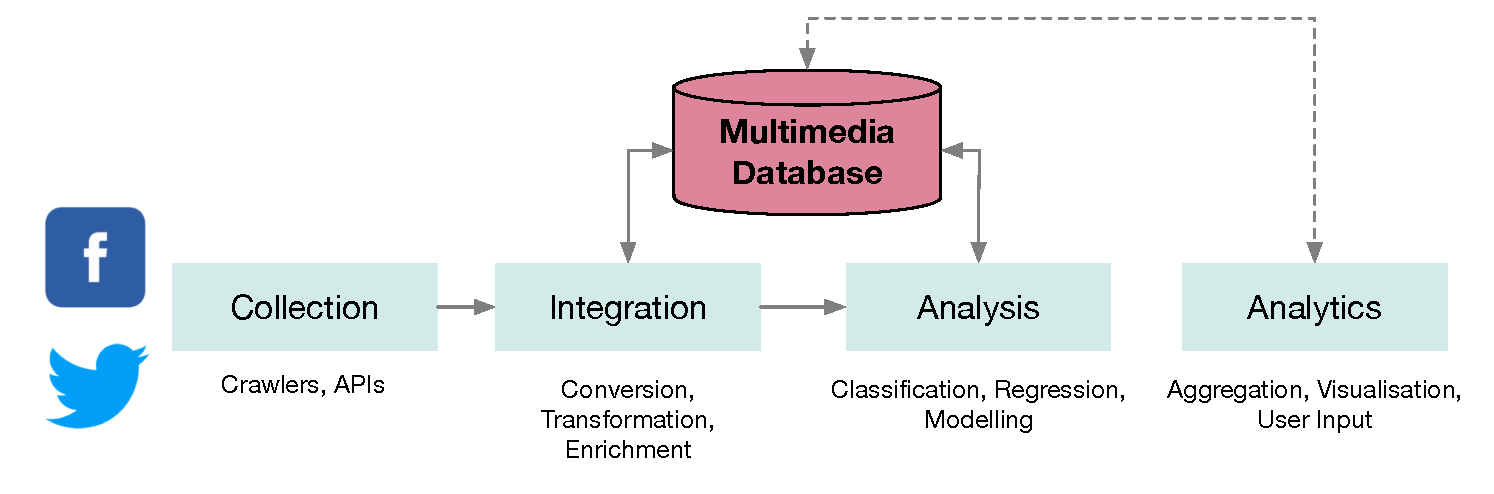
\includegraphics[width=0.90\textwidth]{figures/social-media-architecture.eps}
    \caption{The architecture of a fictious social media analytics platform.}
    \label{figure:social-media}
\end{figure}

Firstly, this database must be able to deal with changing, non-static data, since the various sources will potentially generate a steady and continuous flow of information and so will the analysis and analytics components.

Secondly, and similarily to the multimedia retrieval problem, the pipline is likely to deal with structured, semi-structured and unstructured information that must be stored and processed. Therefore, the data model employed by the multimedia database must be able to cope with this variety. 

And finally, with social media being a very classical field for applying multimedia analytics techniques \cite{Pouyanfar:2018,Jonson:2016}, the different tools built upon the multimedia database will probably rely on a wide range of different query workloads, which the database should be able to accomodate.

\section{Use case 3: Signal Analysis in \acrshort{mrf}}
\label{section:application_mrf}

Multimedia retrieval for medical applications has been an important area of research for many decades now \cite{Mueller:2017Retrieval,Mueller:2004Review} and many of the arguments that we have made in \Cref{section:application_retrieval} can be repeated for this specialised sub-domain.

However, in this section, we want to focus on a very specific application, in which we do not consider media in the classical sense but in a broader sense of raw signals stemming from a \acrfull{mri} device.

\acrshort{mri} is a non-invasive, non-ionizing imaging technique that has gained huge importance in various fields of modern medicine. \acrshort{mri} is enabled by \acrfull{nmr}, which was first described by Purcell and Bloch in 1946 \cite{Bloch:1946Nuclear,Purcell:1946Resonance}. The process behind it is roughly illustrated in \Cref{figure:mri}.

\begin{figure}[b]
    \centering
    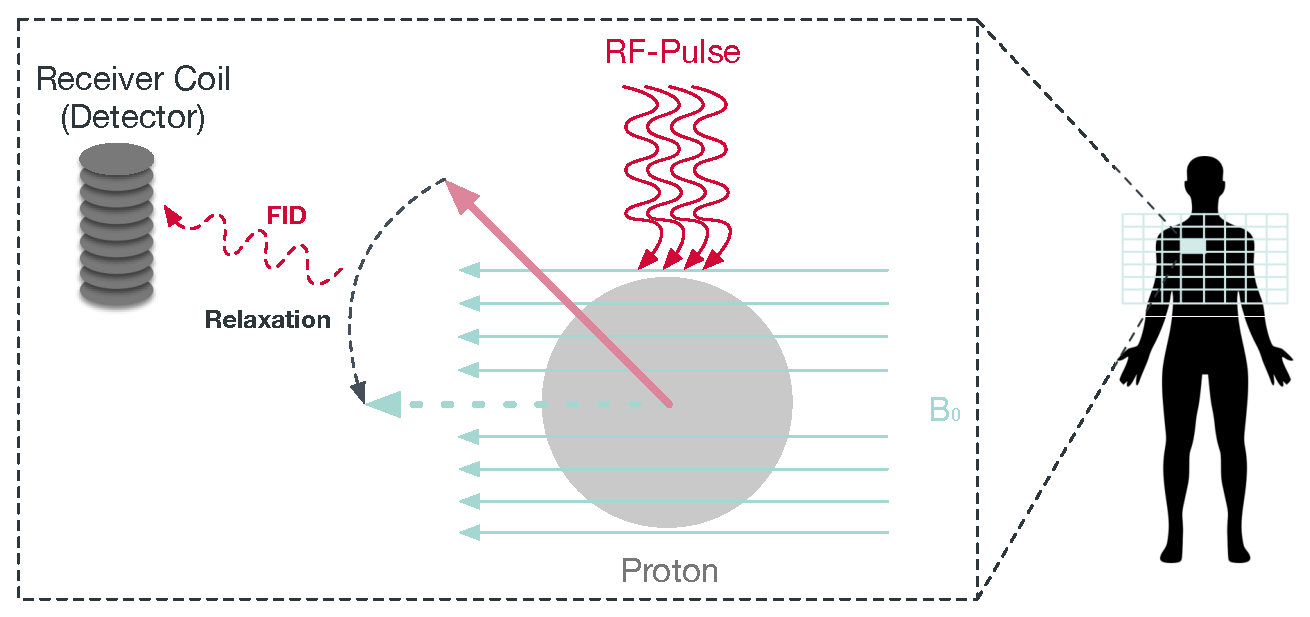
\includegraphics[width=\textwidth]{figures/mri.eps}
    \caption{Simplified illustration of the physical processes enabling \acrshort{mri}.}
    \label{figure:mri}
\end{figure}

In simple terms, an \acrshort{mri}-machine operates by applying a very strong, external, magnetic field -- often referred to as $B_0$ -- which forces nuclei with a non-zero spin, e.g., a $^{1}\text{H}$ nucleus (proton), to align to it. That static field is disrupted by applying a second, radio-frequency pulse that interferes with the nucleus' alignment. As this pulse is switched of, the protons start to re-align with $B_0$ over time in what is called relaxation. This process is characterized by the relaxation times $T_1$ (spin-lattice relaxation) and $T_2$ (spin-spin relaxation), which are specific to a type of material and tissue, and it is accompanied by a measurable, oscillating magnetic field that induces a current in the detector coil. This current -- also known as free induction decay -- is the signal recorded by the \acrshort{mri}-machine and it can be used to reconstruct magnetic properties of the material. Spatial resolution is atained by repeating the entire procedure while scanning a bodypart.

\acrshort{mri} has the ability to generate fine-grained contrasts in different types of soft tissue. However, it comes with two critical disadvantages: Firstly, there is an inherently long acquisition time that can range anything from several minutes to over an hour per scan, especially when one tries to achieve quantification of magnetic properties of soft tissue. Secondly, and due to this lack of fast, quantitative tools, MRI images have become mostly qualitative in nature. Anatomical areas are often referred to as either ``hyperintense'' or ``hypointense'' with respect to their immediate surrounding, but the difference between such areas or even the absolute values themselves cannot be measured directly.

\acrfull{mrf} is a technique \cite{Ma:2013Magnetic} that proposes a solution to this problem and allows for a quantitative mapping of multiple properties simultaneously. The method is described in \cite{Bipin:2019Magnetic} and illustrated in \Cref{figure:mrf}. In summary, \acrshort{mrf} is based on the assumption that different types of tissue produce a distinct signal evolution -- called \emph{fingerprint} -- when exposed a specific acquisition scheme. This means that during data acquisition, measurements take place under varying (pseudo-random), external magnetic field and RF-pulse configurations and signals are recorded for the different configurations resulting in the fingerprint. That fingerprint can then be matched against a database (called dictionary) of pre-calculated, discretised fingerprints that have been simulated using \emph{Bloch}'s theorem of magnetic resonance \cite{Bloch:1946Nuclear}. Through that matching step, values for $B_0$, $T_1$ and $T_2$ (and other parameters) can be obtained and subsequently used to reconstruct an image. Similarily to \acrshort{mri}, spatial resolution is attained by scanning and the overall process is therefore repeated several times.

\begin{figure}[tb]
    \centering
    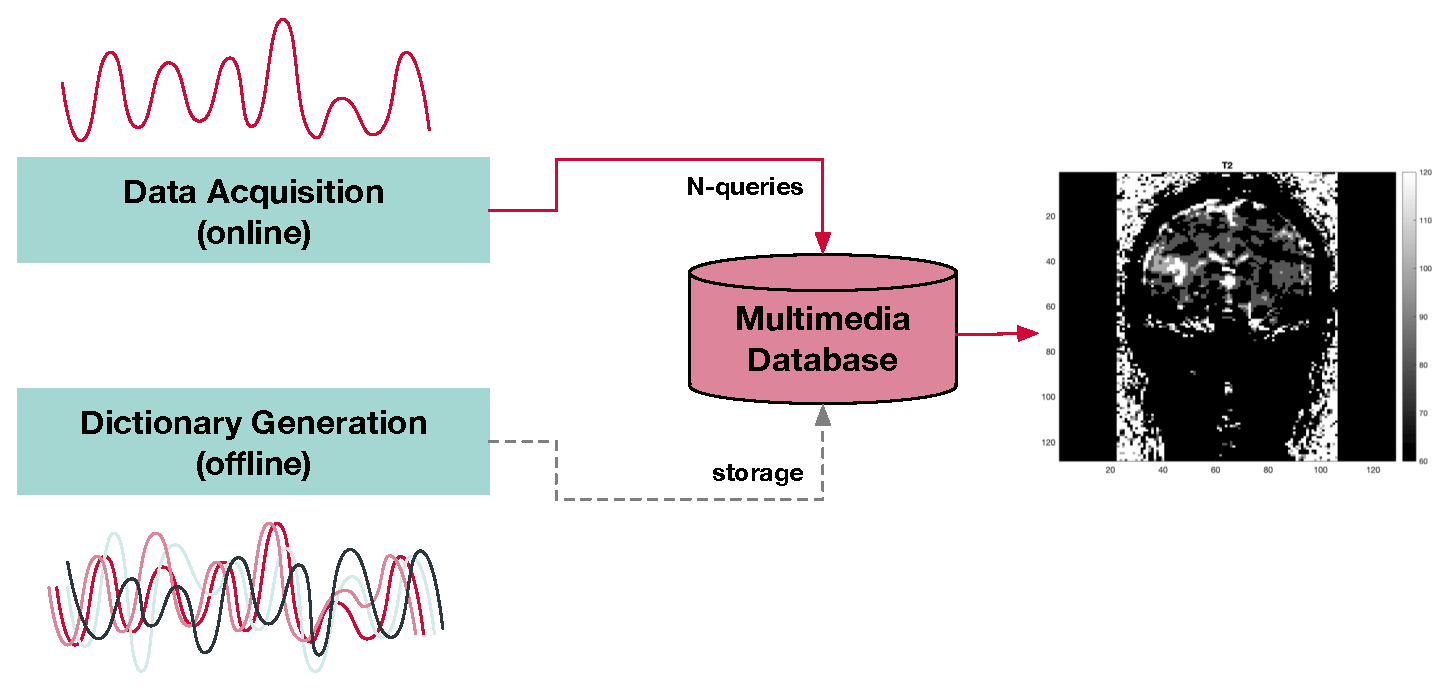
\includegraphics[width=\textwidth]{figures/mrf.eps}
    \caption{Simplified block diagram of a \acrshort{mrf} system (adapted from \cite{Bipin:2019Magnetic}, reconstruction of brain scan kindly provided by Manuel Hürbin).}
    \label{figure:mrf}
\end{figure}

Most implementations realise the pattern matching step as an exhaustive search which obtains the simulated entry from the dictionary that maximises the inner product with the actual signal \cite{Bipin:2019Magnetic}. This is called \acrfull{mips} and it involves obtaining the inner product between a complex signal vector and all the simulated, complex signals. This is a problem similar to the similarity search problem that we solve in multimedia retrieval, with the difference that the vectors compared are complex and not real-valued and that we are only interested in a single result per query. Also similarily to multimedia retrieval, this step is one of the major bottlenecks of the entire process and in fact, several attempts at speeding it up have been made over the years \cite{Mcgivney:2014SVD}\todo{A few more references}.

For a last time, we can try to describe the requirements on a multimedia database that supports the described process: Firstly, and similarily to the multimedia retrieval problem, we have to acknowledge that we require a different data- and query model to store complex vectors and perform \acrshort{mips}, which even differs from the traditional model applied in multimedia retrieval. At the same time, we also store and access very classical data that fits into the Boolean retrieval model such as the individual parameters $B_0$, $T_1$ and $T_2$. 

Secondly, and also similarily to interactive multimedia retrieval, retrieval time is an important aspect and should be minimised as much as possible. However, in contrast to multimedia retrieval, execution time cannot be bought by sacrificing retrieval quality, because the \acrshort{mrf} problem does have a human in the loop that might correct an error in an individual query.

\section{Deriving Requirements}
In the use-cases presented in Sections \ref{section:application_retrieval}, \ref{section:application_online_analysis} and \ref{section:application_mrf} we have discussed three applications that, 
\begin{enumerate*}[label=(\roman*)]
    \item deal with large amounts of unstructured (multimedia) data that must be stored and managed,
    \item use some mathematical descriptors of that unstructured (multimedia) data to enable analysis, comparison and queries,
    \item and that combine these descriptors with data such as labels, descriptions and other information, that must be accessed and sometimes queried as well.
\end{enumerate*}

We acknowledge, that while the details may vary, the basic needs outlined in the aforementioned use-cases are overlaping to such an extent that it raises the question whether a dedicated multimedia database management system would make sense. In fact, the argument for such a system has been made by different authors before us \cite{Smeulders:2000Content,Zahalka:2014towards,Jonson:2016} and steps towards such a system have been taken \cite{Giangreco:2018Database,Wang:2021Milvus}. However, all concrete approaches somehow narrow the scope in a way that restricts their generalisability.

In this section, we therefore try to formalise the requirements for such a general-purpose multimedia database system.

\subsection{Complex Data Types as First-class Citizen}
Due to the reliance of multimedia analysis and analytics workloads on mathematical objects such as vectors, complex numbers or matrices, we argue, that the data model of a multimedia database must be extended to consider those types of data as \emph{first-class citizens} in addition to well-established data types such as numbers, strings and other scalars. This means, that the structure as well as the mathematical properties of those types must be considered for query planning and execution.

This is not a new idea, per-se, and to some extent self-evident since new use-cases obiously require additions to existing data models. Therefore, unsurprisingly, the idea of extensible data models was already discussed as early as 1988 \cite{Linnemann:1988Design}. Similarily, it was also proposed by \cite{Giangreco:2018Database} that in order to support multimedia retrieval workloads in a relational database, one must (among other things) extend the relational model to support those vectors. 

However, to the best of our knowledge, existing solutions fall short of offering that support in a manner that allows the multimedia database to be aware of how such objects can be stored and operated upon efficiently, given not only structural but also mathematical properties.

\begin{requirement}[label=requirement:complex_data_types]{Complex Data Types as First-class Citizen}{}
    A multimedia database must treat composite data types that serve a mathematical purpose (e.g., vectors, complex numbers, matrices, tensors) as first-class citizens of the data model in addition to primitive types such as simple numbers or strings.
\end{requirement}

\subsection{Functions as First-class Citizen}

All multimedia retrieval problems considered so far involve the execution of functions that operate on the individual data items, e.g., to determine the similarity or the inner product between items in the database. For a multimedia database to be able to operate efficiently, those functions must be considered first-class citizens of the data model as well, in that the multimedia database must have the ability to reason about them and make decisions regarding their execution.

A database supporting \acrshort{sql}, for example, only provides very basic functions outlined in the \acrshort{sql}-standard \cite{XOpen:1996SQL} as part of the query language. Those are not sufficient to accomodate the workloads described in this chapter. 

\begin{requirement}{Functions as First-class Citizen}{}
    A multimedia database must treat certain mathematical functions as first-class citizens and must have the ability to reason about those functions properties during query-planning and execution.
\end{requirement}

\subsection{High-Dimensional Indexing}

In order to support fast multimedia analysis and analytics, novel indexing strategies must be supported to provide efficient access to the complex data types and values derived from them. This is a well-known issue 

\begin{requirement}{High-dimensional Indexing}{}
    A multimedia database must treat certain functions as first-class citizens of the data model with the ability to reason about their properties during query-planning and execution.
\end{requirement}

\subsection{Functions as First-class Citizen}

All multimedia retrieval problems considered so far involve the execution of functions that operate on the individual data items, e.g., to determine the similarity or the inner product. For a multimedia database to be able to operate efficiently, those functions must be considered first-class citizens of the data model as well, in that the multimedia database must have the ability to reason about them and make decisions regarding their execution.

\begin{requirement}{Functions as First-class Citizen}{}
    A multimedia database must treat certain functions as first-class citizens of the data model with the ability to reason about their properties during query-planning and execution.
\end{requirement}